


\documentclass[a4paper,12pt]{article}
\usepackage{amsmath}
\usepackage{tikz}
\usetikzlibrary{arrows.meta}
\usetikzlibrary{positioning}
\usepackage{hyperref}
\usepackage{geometry}
\geometry{margin=1in}
\title{Worksheet 6 - outline solutions}

\author{Conor Houghton, copying from Martha Lewis}
\date{}

\begin{document}

\maketitle

\section*{Search Problems}

\textbf{Question 1.} Consider the search tree shown below. The numbers on the branches are the costs.
\begin{center}
  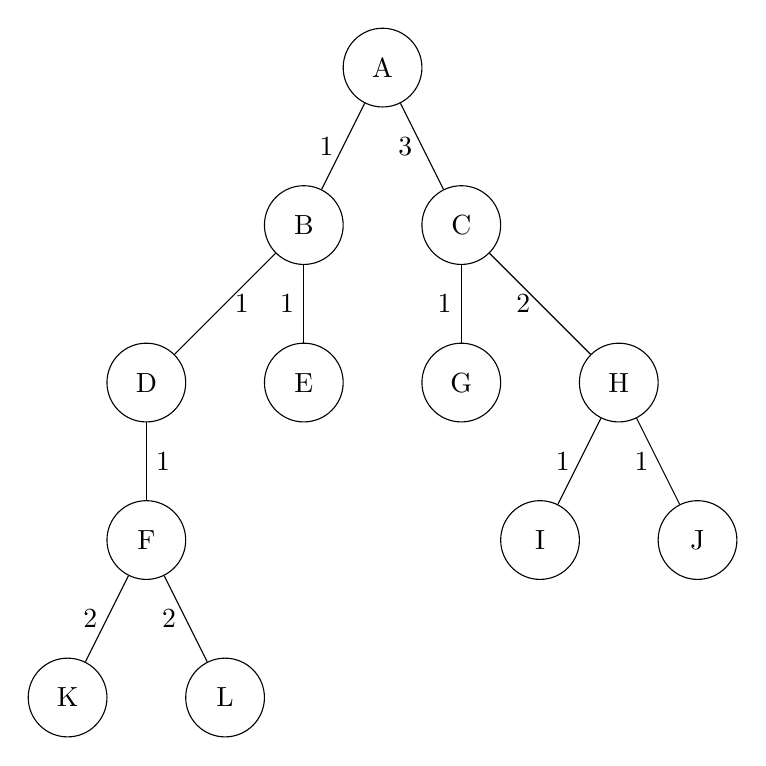
\begin{tikzpicture}[scale=1]
\tikzset{
    leaf/.style={
              circle,
                   draw,
                   minimum size=1cm
    }
}
    \node (A)[leaf] at (-1,0) {A};
    \node (B)[leaf] at (-2,-2) {B};
    \node (C)[leaf] at (0,-2) {C};
    \node (D)[leaf] at (-4,-4) {D};
    \node (E)[leaf] at (-2,-4) {E};
    \node (G)[leaf] at (0,-4) {G};
    \node (H)[leaf] at (2,-4) {H};
    \node (F)[leaf] at (-4,-6) {F};
    \node (I)[leaf] at (1,-6) {I};
    \node (J)[leaf] at (3,-6) {J};
    \node (K)[leaf] at (-5,-8) {K};
    \node (L)[leaf] at (-3,-8) {L};

    \draw (A) -- node[left] {$1$} (B);
    \draw (A) -- node[left] {$3$} (C);
    \draw (B) -- node[right] {$1$} (D);
    \draw (B) -- node[left] {$1$} (E);
    \draw (C) -- node[left] {$1$} (G);
    \draw (C) -- node[left] {$2$} (H);
    \draw (D) -- node[right] {$1$} (F);
    \draw (H) -- node[left] {$1$} (I);
    \draw (H) -- node[left] {$1$} (J);
    \draw (F) -- node[left] {$2$} (K);
    \draw (F) -- node[left] {$2$} (L);

\end{tikzpicture}
\end{center}

Assume that the nodes are expanded in alphabetical order when no other order is specified by the search, and that the goal is state G. What order would the states be expanded by each type of search? Stop when you expand G.

\begin{enumerate}
    \item Depth First: \textsl{solution} ABDFKLECG
    \item Breadth First: \textsl{solution} ABCDEG
    \item Uniform Cost Search: \textsl{solution} ABDECFG
\end{enumerate}

\noindent \textbf{Question 2.} Consider the water jugs problem. You have a tap, a 5-litre bucket, and a 7-litre bucket. You need \textbf{EXACTLY} 4 litres of water. You may fill either bucket from the tap or the other bucket; you may empty either bucket into the drain or into the other bucket.

\begin{enumerate}
    \item What are the actions possible in a state where you have $S$ litres of water in the small bucket and $L$ litres in the large bucket? \textsl{solution} The actions are: fill bucket 1, fill bucket 2, empty bucket 1, empty bucket 2, pour bucket 1 into bucket 2, pour bucket 2 into bucket 1.
    \item Starting from the initial state (0,0), draw the search tree until you reach a goal node, with 4 litres of water in one or other of the buckets. \textsl{solution}: leaving out nodes that were already visited:

\begin{center}

\begin{tikzpicture}[
    every node/.style={draw, circle, minimum size=0.8cm, align=center},
    level distance=2cm,
    level 1/.style={sibling distance=4cm},
    level 2/.style={sibling distance=2cm},
    level 3/.style={sibling distance=1.5cm},
    level 4/.style={sibling distance=1cm},
    edge from parent/.style={draw, ->, >=stealth}
]

    % Root node
    \node (root) at (0, 0) {0, 0};

    % Level 1: Fill 5L or Fill 7L
    \node[below left=of root] (50) {5, 0};
    \node[below right=of root] (07) {0, 7};

    \draw (root) -- (50) ;%node[midway, left] {Fill 5L};
    \draw (root) -- (07) ;%node[midway, right] {Fill 7L};

    % Level 2: From (5, 0)
    \node[below left=of 50] (05) {0, 5};
    \node[below right=of 50] (57) {5, 7};

    \draw (50) -- (05) ;
    \draw (50) -- (57) ;
    
    % Level 2: From (0, 7)
    \node[below right=of 07] (52) {5, 2};

    \draw (07) -- (52) ;%node[midway, left] {Pour 7L->5L};

    `%level 3: from (0,5)
    \node[below right=of 05] (55) {5, 5};
    \draw (05) -- (55);
    
    `%level 4: from (5,5)
    \node[below=of 55] (37) {3, 7};
    \draw (55) -- (37);

    
\end{tikzpicture}
\end{center}
After this the tree just follows the two branches down, on the left
$$3,7\rightarrow 3,0 \rightarrow 0,3 \rightarrow 5,3 \rightarrow 1,7 \rightarrow 1,0 \rightarrow 0,1 \rightarrow 5,1 \rightarrow 0,6 \rightarrow 5,6 \rightarrow 4,7$$
and on the right
$$5,2\rightarrow 0,2\rightarrow 2,0 \rightarrow 2,7 \rightarrow 5,4$$

    \item Would breadth or depth-first search be best to find the optimal solution? Why? \textsl{solution}: Breadth first search would find the optimal solution, since we can view each action as
having the same cost, whereas depth-first search could find a solution that would take
longer.
\end{enumerate}

\noindent \textbf{Question 3.} Below is a graph to be searched (from node S to node G).
\begin{center}
  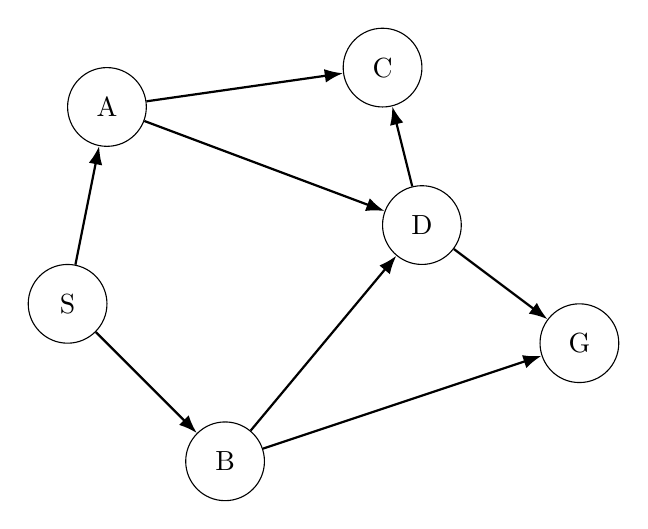
\begin{tikzpicture}[scale=1]
\tikzset{
  thisNode/.style={
    circle,
                   draw,
                   minimum size=1cm
    }
}
    \node (A)[thisNode] at (-3.5,0.5) {A};
    \node (C)[thisNode] at (0,1) {C};
    \node (D)[thisNode] at (0.5,-1) {D};
    \node (S)[thisNode] at (-4,-2) {S};
    \node (B)[thisNode] at (-2,-4) {B};
    \node (G)[thisNode] at (2.5,-2.5) {G};

    \draw[->, thick, >=Latex] (A) -- (C);
    \draw[->, thick, >=Latex] (A) -- (D);
    \draw[->, thick, >=Latex] (D) -- (C);
    \draw[->, thick, >=Latex] (D) -- (G);
    \draw[->, thick, >=Latex] (S) -- (A);
    \draw[->, thick, >=Latex] (S) -- (B);
    \draw[->, thick, >=Latex] (B) -- (D);
    \draw[->, thick, >=Latex] (B) -- (G);

    
\end{tikzpicture}
\end{center}




You are given a list of heuristic estimates at the states:
\begin{align*}
    A &= 2 \\
    B &= 3 \\
    C &= 1 \\
    D &= 4 \\
    S &= 10 \\
    G &= 0
\end{align*}
Break ties using alphabetical order. Perform a best-first greedy search. Show the path to the goal. \textsl{solution}: Best first greedy search would expand nodes in the following order: A, C, D, G. The path found
is SADG.\\[1 cm]



\noindent \textbf{Question 4.} We are given the following graph, where each node has an identifier and a heuristic value, while each edge has a cost.
\begin{center}
  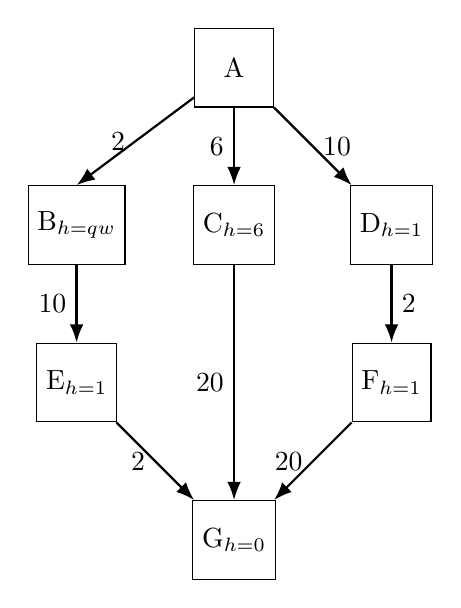
\begin{tikzpicture}[scale=1]
\tikzset{
    thisNode/.style={
                   draw,
                   minimum size=1cm
    }
}
    \node (A)[thisNode] at (0,0) {A};
    \node (B)[thisNode] at (-2,-2) {B$_{h=qw}$};
    \node (C)[thisNode] at (0,-2) {C$_{h=6}$};
    \node (D)[thisNode] at (2,-2) {D$_{h=1}$};
    \node (E)[thisNode] at (-2,-4) {E$_{h=1}$};
    \node (F)[thisNode] at (2,-4) {F$_{h=1}$};
    \node (G)[thisNode] at (0,-6) {G$_{h=0}$};

    \draw[->, thick, >=Latex] (A) -- node[left] {2} (B.north);
    \draw[->, thick, >=Latex] (A) -- node[left] {6} (C.north);
    \draw[->, thick, >=Latex] (A) -- node[right] {10} (D);
    \draw[->, thick, >=Latex] (B) -- node[left] {10} (E);
    \draw[->, thick, >=Latex] (C) -- node[left] {20} (G);
    \draw[->, thick, >=Latex] (D) -- node[right] {2} (F);
    \draw[->, thick, >=Latex] (E) -- node[left] {2} (G);
    \draw[->, thick, >=Latex] (F) -- node[left] {20} (G);

    
\end{tikzpicture}
\end{center}


\begin{enumerate}
    \item Show the order in which A* search sees nodes from S to G (goal node). For each node during the search, show its $f$ and $g$ values. If a node is reached on multiple paths, show its $f$ and $g$ values each time the node is reached, and indicate its parent node.
    \item What is the solution path found?
    \item Is the $h$ function admissible? Is it consistent?
    \item Suppose you decide to do best-first search using the following evaluation function:
    \begin{equation*}
        f(n) = (1 - w) g(n) + w h(n)
    \end{equation*}
    Assuming that $h(n)$ is admissible, what are the values of $w$ that guarantee the algorithm will find an optimal solution?
\end{enumerate}

\textsl{solution}: So from A all the connected nodes are updated to
give B:2, C:6 and D:11; the distance plus heuristic is therefore using a notation I have just made up but which is hopefully clear:
B:$f$14, C:$f$12 and D:$f$11 and as such D is the next noded visited. The
only connected node is F and so we update F:12 and F:$f$13. This means
the next node to visit is C giving G:26. Now we go D making E:12 and
E:$f$13. If we break the tie alphabetically we go to E next giving
G:14. We need to check F but that doesn't change anything and the
final goal is now the nearest node with path ABEG. What a useless
heuristic! Yes, $h$ is admissible. No, $h$ is not consistent. To see
why we can look for decreasing f values on any path. The triangle
inequality is violated for nodes B and E. With $w = 0$ the algorithm
is uniform cost, which is guaranteed to find an optimal solution if
there is a solution.  With $w = 0.5$ the algorithm is A-star, which,
given that h is admissible, is guaranteed to find an optimal solution
if there is a solution.


\end{document}
